\subsection{强监督分割方法}
%%%
\begin{frame}{强监督分割方法}
\begin{center}
``写在前面:{\color{red}非原创工作均有标注引用}''
\end{center}
\begin{columns}[c]
\column{.6\textwidth}
\begin{figure}
    \centering
    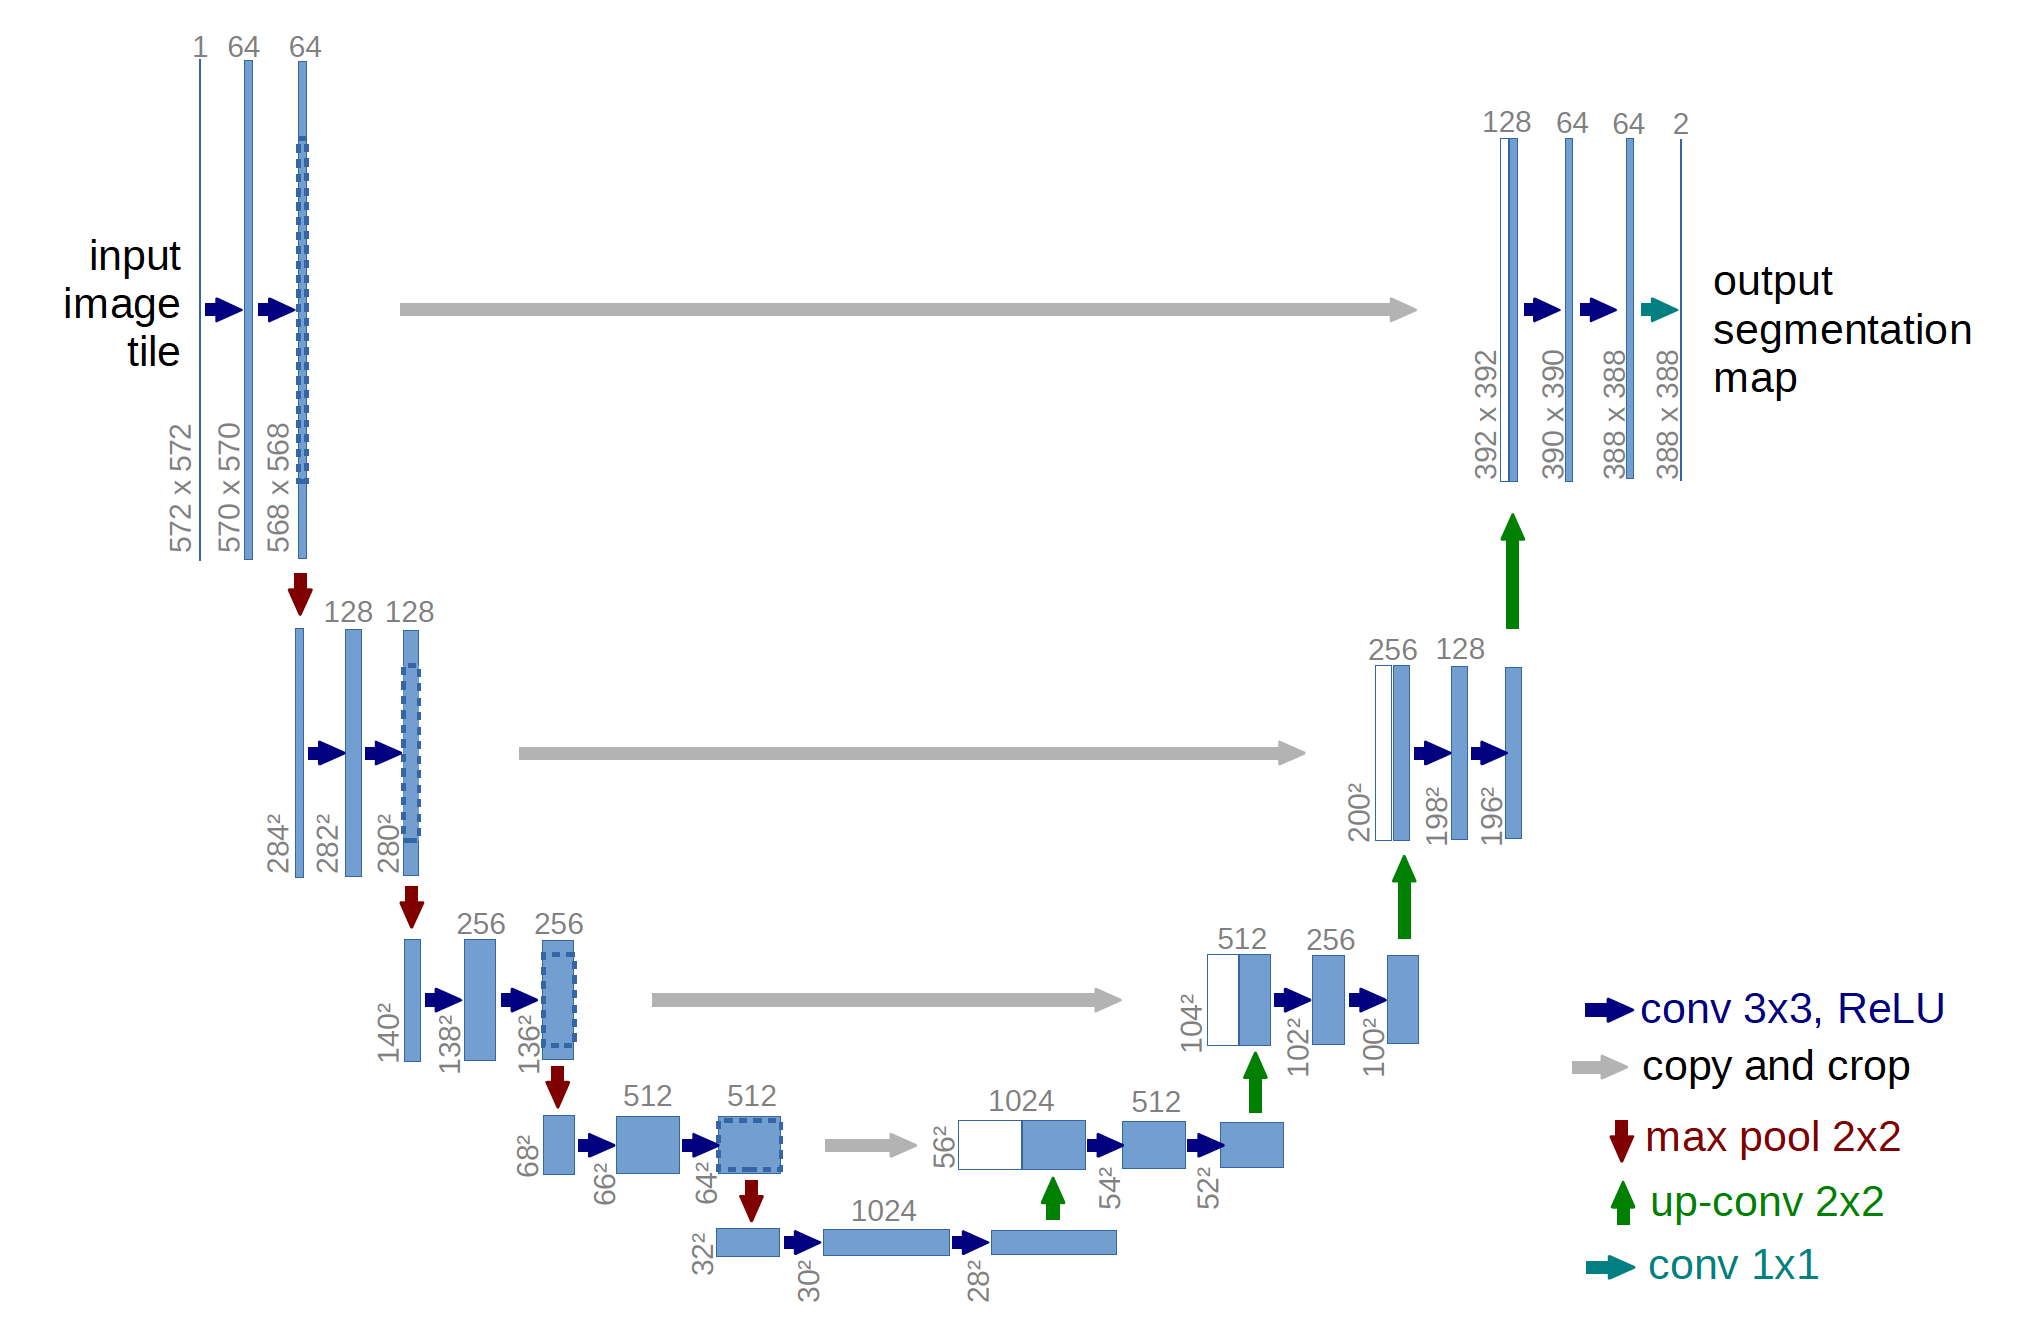
\includegraphics[width=\linewidth]{figures/chap2_Unet.png}
    \caption{编码器-解码器结构\footnote[frame]{\tiny O. Ronneberger, et al. U-net: Convolutional networks for biomedical image segmentation. In International Conference on Medical image computing and computer-assisted intervention, pages 234–241. Springer, 2015.}}
\end{figure}

\column{.5\textwidth}
\begin{itemize}
\item 监督方式:强监督 \pause
\item ``人工智能,有多少智能,就有多少人工''
\item $\Rightarrow$~Vit2019数据集
\end{itemize}
\end{columns}
\end{frame}
%%%
\begin{frame}{数据集Vit2019}
\begin{columns}[c]
\column{.6\textwidth}
\begin{figure}
    \centering
    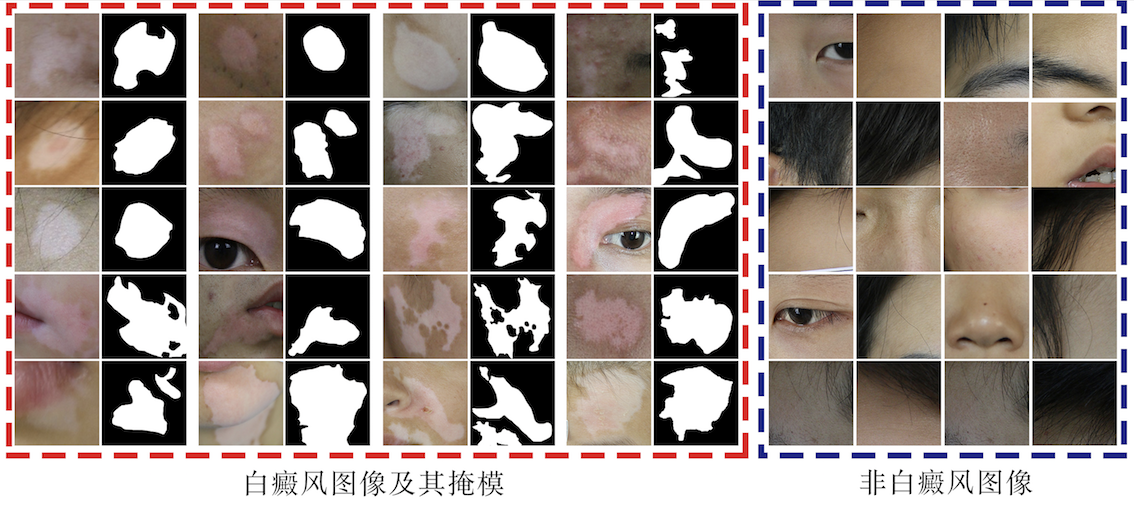
\includegraphics[width=\linewidth]{figures/chap2_DatasetGragh1.png}
    \caption{Vit2019数据集}
\end{figure}

\column{.5\textwidth}
\begin{itemize}
\item 规模:1000+1000
\item 标注:像素级标注
\item 多样性:光照、肤色、不同治疗阶段等
\end{itemize}
\end{columns}

\end{frame}
%%%
\begin{frame}{数据集Vit2019的挑战}
\begin{columns}[c]
\column{.5\textwidth}
\begin{figure}
    \centering
    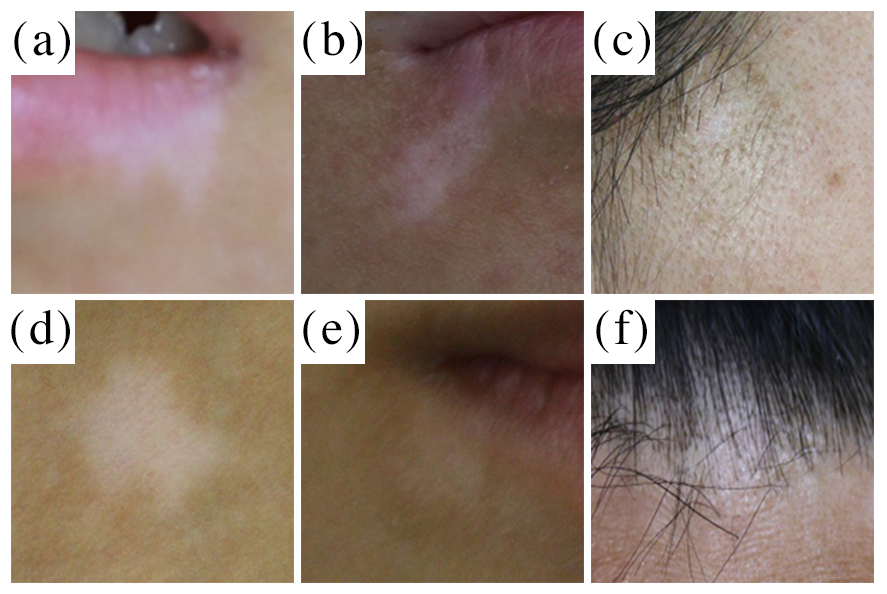
\includegraphics[width=\linewidth]{figures/chap1_challenge.jpg}
\end{figure}

\column{.5\textwidth}
\begin{itemize}
\item 肤色差别大((a) vs. (b))
\item 对比度低((a) , (e))
\item 毛发影响((c) , (f))
\item 局部高光(易误判)((c))
\end{itemize}
\end{columns}
\end{frame}
%%%
\begin{frame}{Baseline: Unet\footnote[frame]{\tiny O. Ronneberger, et al. U-net: Convolutional networks for biomedical image segmentation. In
International Conference on Medical image computing and computer-assisted intervention, pages 234–241. Springer, 2015.}}
\begin{columns}[c]
\column{.5\textwidth}
\begin{figure}
    \centering
    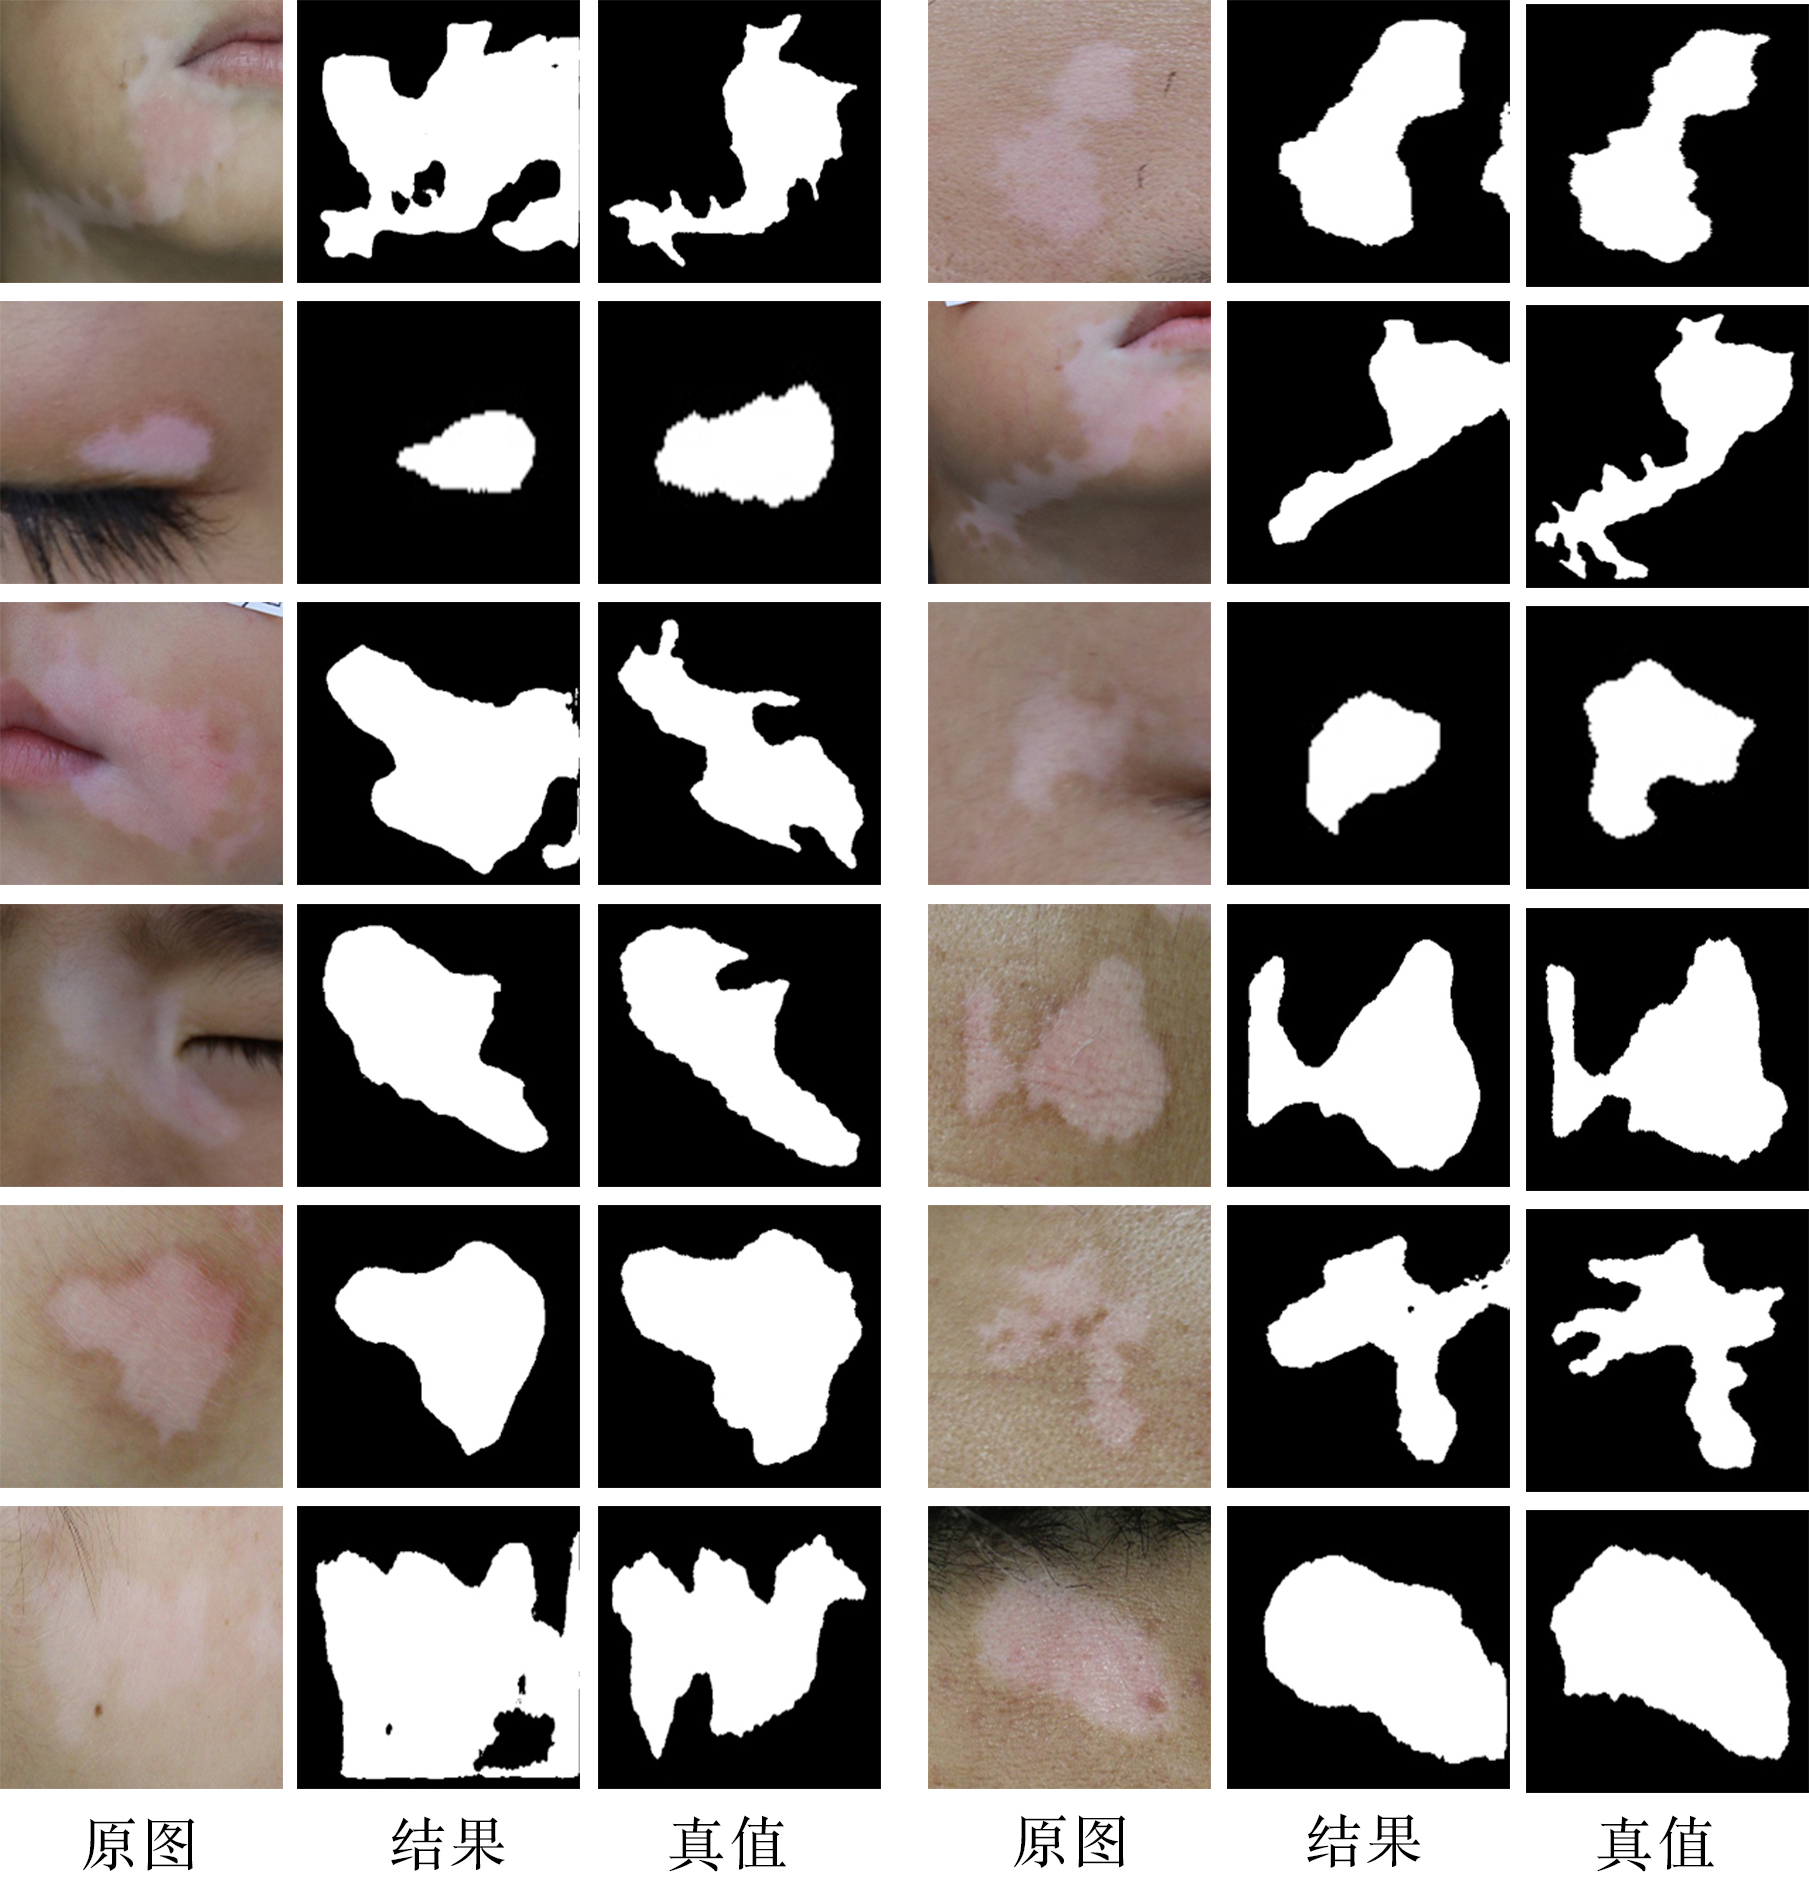
\includegraphics[width=\linewidth]{figures/UnetResult.jpg}
\end{figure}

\column{.45\textwidth}

\begin{IEEEeqnarray}{rCl}
\label{eq:1}
\mathrm{IoU}=&&\frac{\mathrm {Area\,of\,Overlap}}{\mathrm {Area\,of\,Union}} \nonumber \\
\nonumber \\ 
=&&78.6\% \nonumber
\end{IEEEeqnarray}
\begin{itemize}
\item 强监督方法局限性: \\ 数据标注工作耗时耗力
\end{itemize}
\end{columns}
\end{frame}
%%%
\subsection{弱监督分割方法}
\begin{frame}{弱监督分割框架}
\begin{figure}
    \centering
    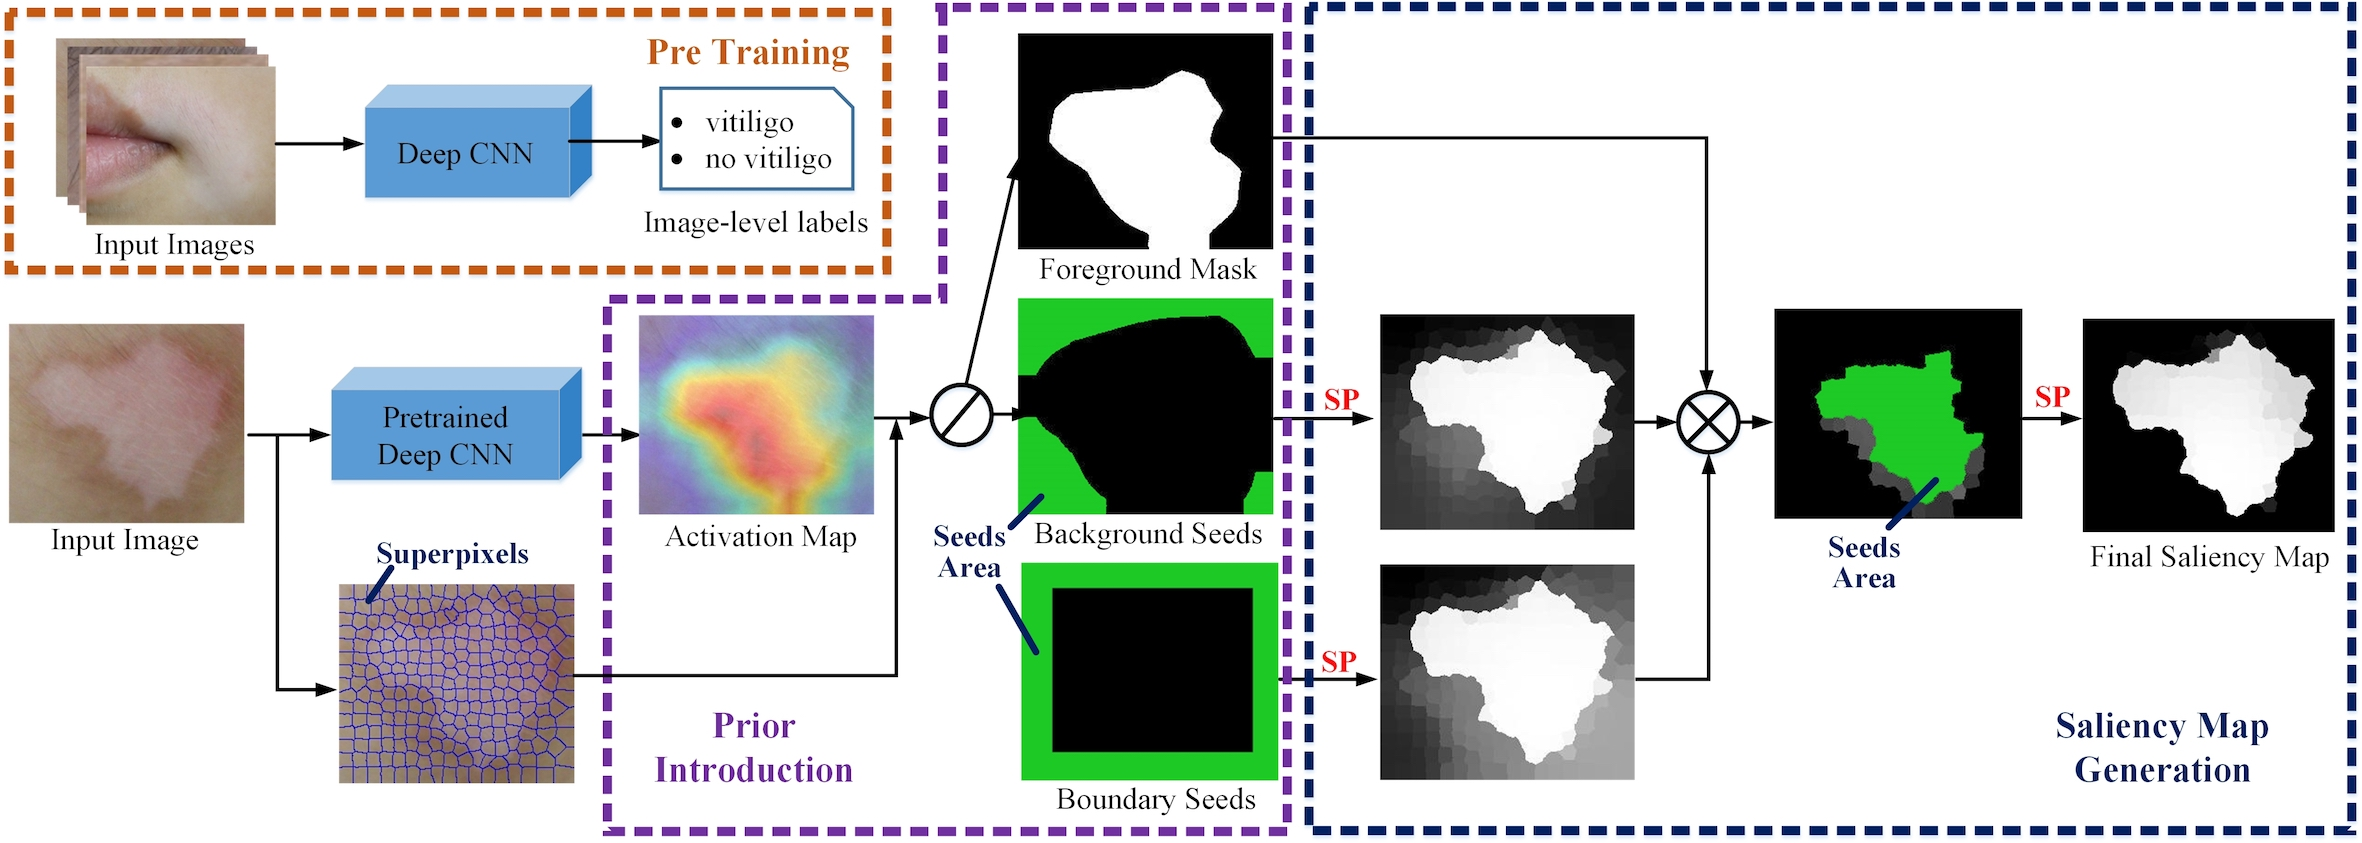
\includegraphics[width=\linewidth]{figures/CNNandSuperPixelModelGraph3.jpg}
\end{figure}
\vfill
\begin{itemize}
\item 超像素分割
\item 高层语义特征+底层特征 ---``既见树木,又见森林''
\item 将反馈应用于显著性传播过程
\end{itemize}
\end{frame}
%%%

\begin{frame}{超像素分割}
\begin{columns}[c]
\column{.6\textwidth}
\begin{figure}
    \centering
    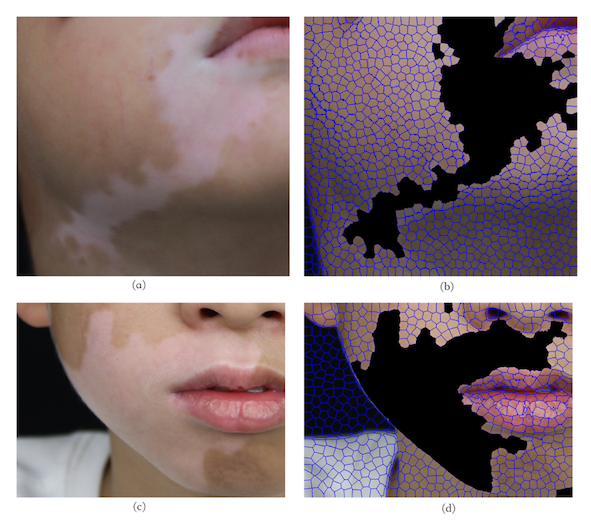
\includegraphics[width=\linewidth]{figures/chap3_SLICresult2.png}
\end{figure}

\column{.45\textwidth}
好处:
\begin{itemize}
\item 降低数据维度
\item 剔除异常像素点
\item 保留较完整的皮损边界
\end{itemize}
\end{columns}
\end{frame}
%%%
\begin{frame}{``既见树木,又见森林''}
\begin{block}{定义}
``森林'': 高层特征 $\Rightarrow$ 定位种子区域

``树木'':底层特征 $\Rightarrow$ 传播
\end{block}

\vfill 
\pause
\begin{itemize}
\item 定位:类激活图\footnote[frame]{\tiny Zhou, Bolei, et al. Learning deep features for discriminative localization. CVPR 2016.} ( {\color{red}C}lass {\color{red}A}ctivation {\color{red}M}ap -- {\color{red}CAM})
\begin{figure}
    \centering
    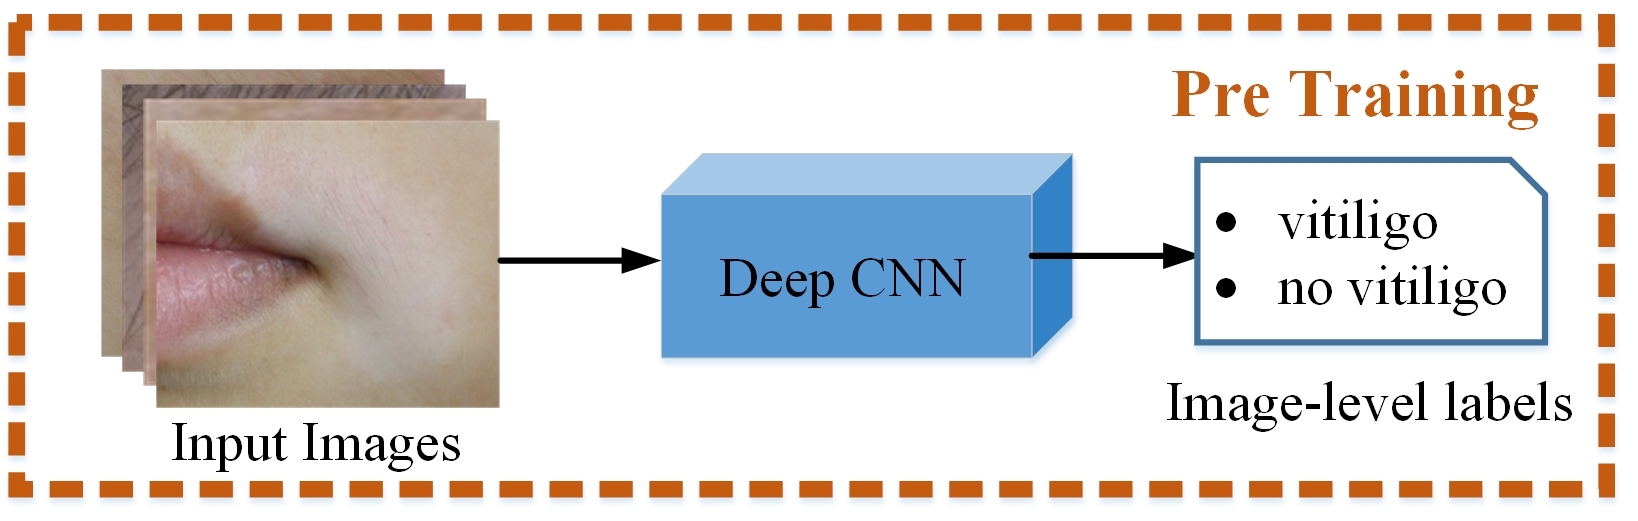
\includegraphics[width=0.5\linewidth]{figures/TrainForCam.jpg}
\end{figure}
\end{itemize}

\vspace{-0.2cm}

\begin{figure}
    \centering
    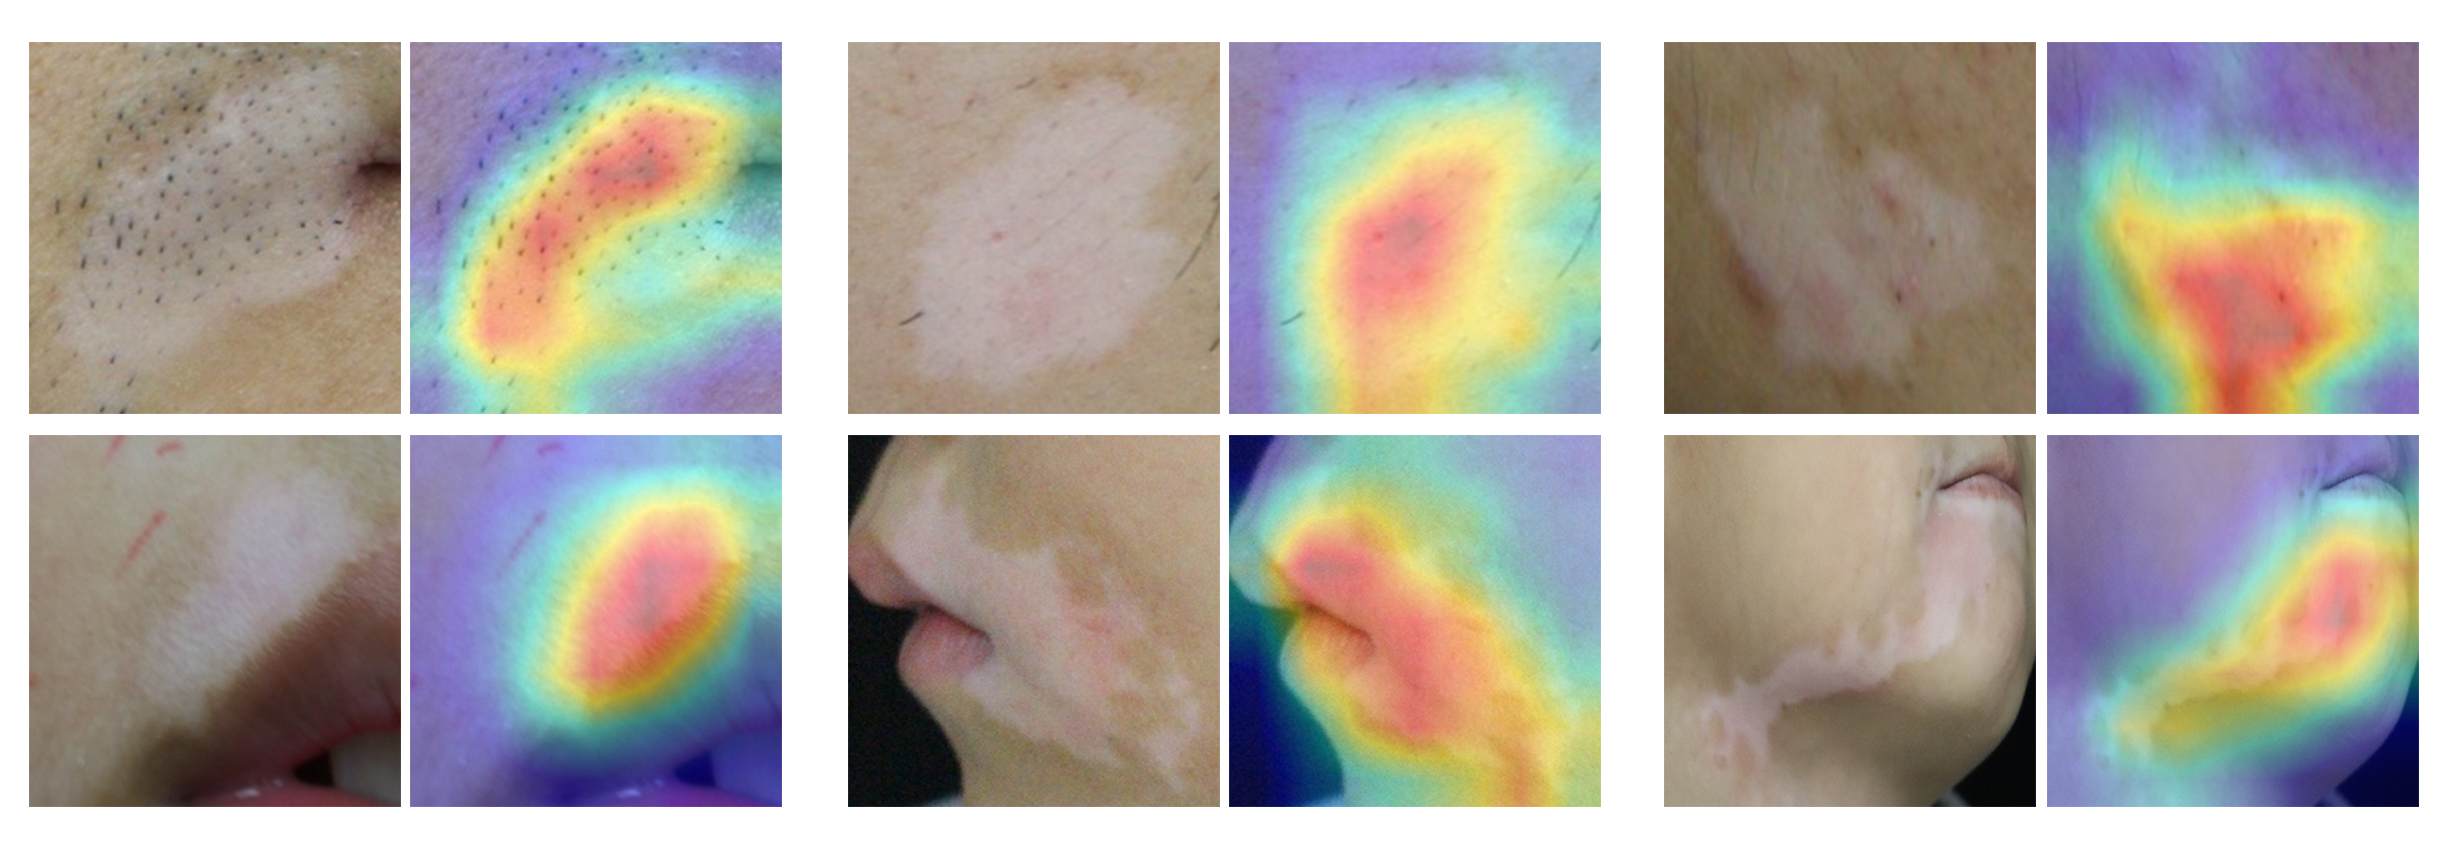
\includegraphics[width=0.65\linewidth]{figures/cam.jpg}
\end{figure}

\end{frame}
%%%
\begin{frame}{``既见树木,又见森林''}
\begin{block}{定义}
``森林'': 高层特征 $\Rightarrow$ 定位种子区域

``树木'':底层特征 $\Rightarrow$ 传播
\end{block}
\vfill
传播:
\begin{columns}[c]
\column{.6\textwidth}
\begin{figure}
    \centering
    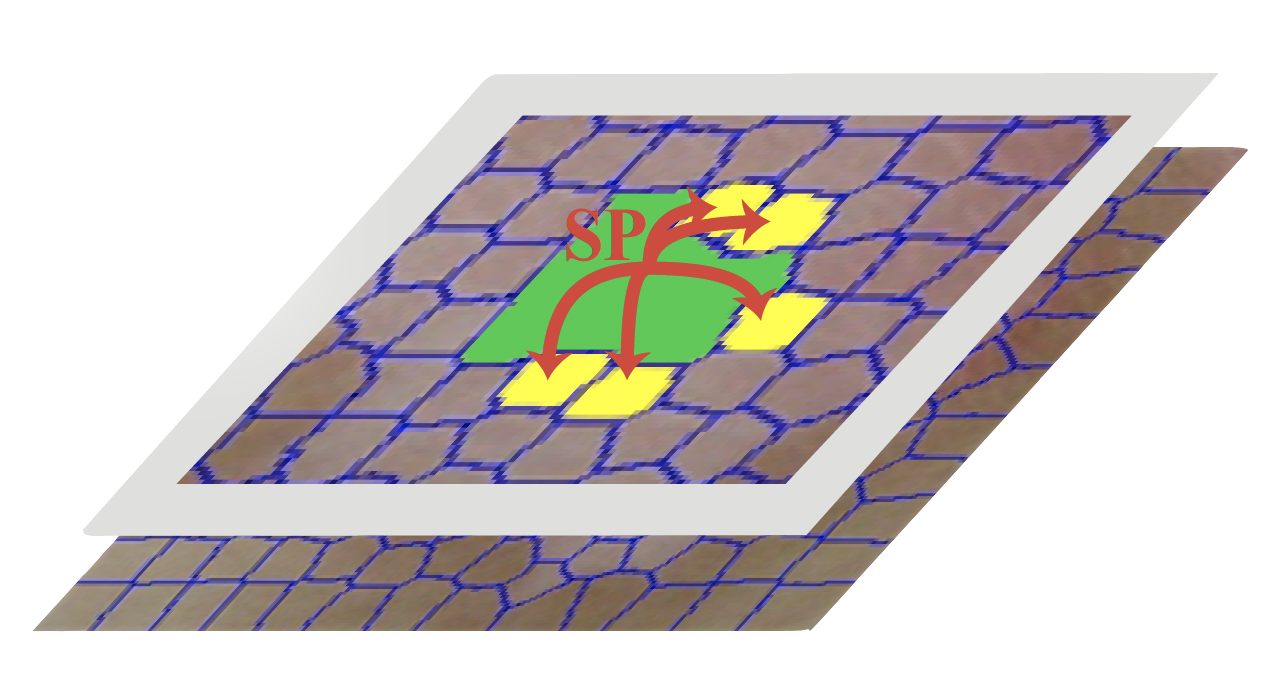
\includegraphics[width=.9\linewidth]{figures/propagationillustrator.png}
\end{figure}

\column{.5\textwidth}
\begin{itemize}
\item 传播过程迭代化
\item 每一次迭代需要确定传播的{\color{blue}{顺序}}\footnote[frame]{\tiny C. Gong et al. Saliency propagation from simple to difficult. CVPR 2015.}和{\color{blue}{数量}}
\end{itemize}
\end{columns}

\end{frame}
%%%
\begin{frame}{``既见树木,又见森林''--传播}

\begin{columns}[c]
\column{.5\textwidth}
\begin{figure}
    \centering
    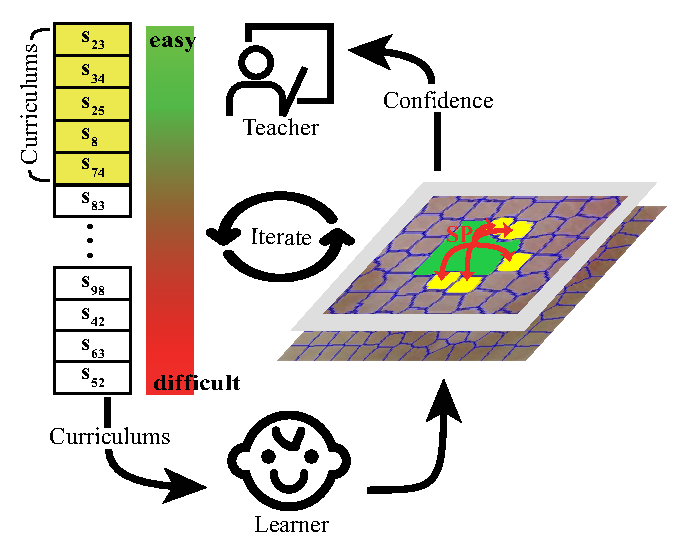
\includegraphics[width=\linewidth]{figures/TLLTillustrator.eps}
    \caption{反馈思想与传播相结合}
\end{figure}

\column{.6\textwidth}
\begin{itemize}
\item 传播过程~$\Rightarrow$~``教学-学习''
\item 老师:
\begin{itemize}
\item 评估课程难度,从易到难布置一定数量的课程;
\item 接受学生反馈
\end{itemize}
\item 学生:
\begin{itemize}
\item 学习课程(传播);
\item 反馈学习效果(confidence)
\end{itemize}
\end{itemize}
\begin{block}{数量}
\small $q^{(t)}={|\mathrm{\#Neighbor^{(t)}}|\times \mathrm{Confidence}^{(t-1)}}$
\end{block}
\end{columns}
\end{frame}
%%%
\begin{frame}{``既见树木,又见森林''--传播}

\begin{block}{老师度量``课程''难度}
$DS_i=INF_i+IND_i+IHM_i+CON_i$
\begin{itemize}
\item 信息性:$INF_i=H(\mathbf{s}_i \mid \mathcal{L})$
\item 个体性:$IND_i=\frac{1}{|\mathcal{N}(\mathbf{s}_i)|}\sum_{j\in \mathcal{N}(\mathbf{s}_i)}\| \mathbf{s}_i^{\mathrm color}-\mathbf{s}_j^{\mathrm color}\|$
\item 同质性:$IHM_i=\Big (\frac{2}{b^2-b}\sum_{i=1}^b \sum_{j=i+1}^b\pmb{\Theta}_{ij}\Big )^{-1}$
\item 连通性:$CON_i=\frac{1}{l}\sum_{j\in \mathcal{L}}\mathrm{geo}({\mathbf{s}_i,\mathbf{s}_j})$
\end{itemize}
\end{block}

\begin{block}{学生反馈效果}
$\mathrm{Confidence}=1-\frac{2}{q^{(t-1)}}\sum_{i=1}^{q^{(t-1)}}\min{(f_i^{(t-1)},1-f_i^{(t-1)})}$
\end{block}
\end{frame}
%%%
\begin{frame}{方法框架}
\begin{figure}
    \centering
    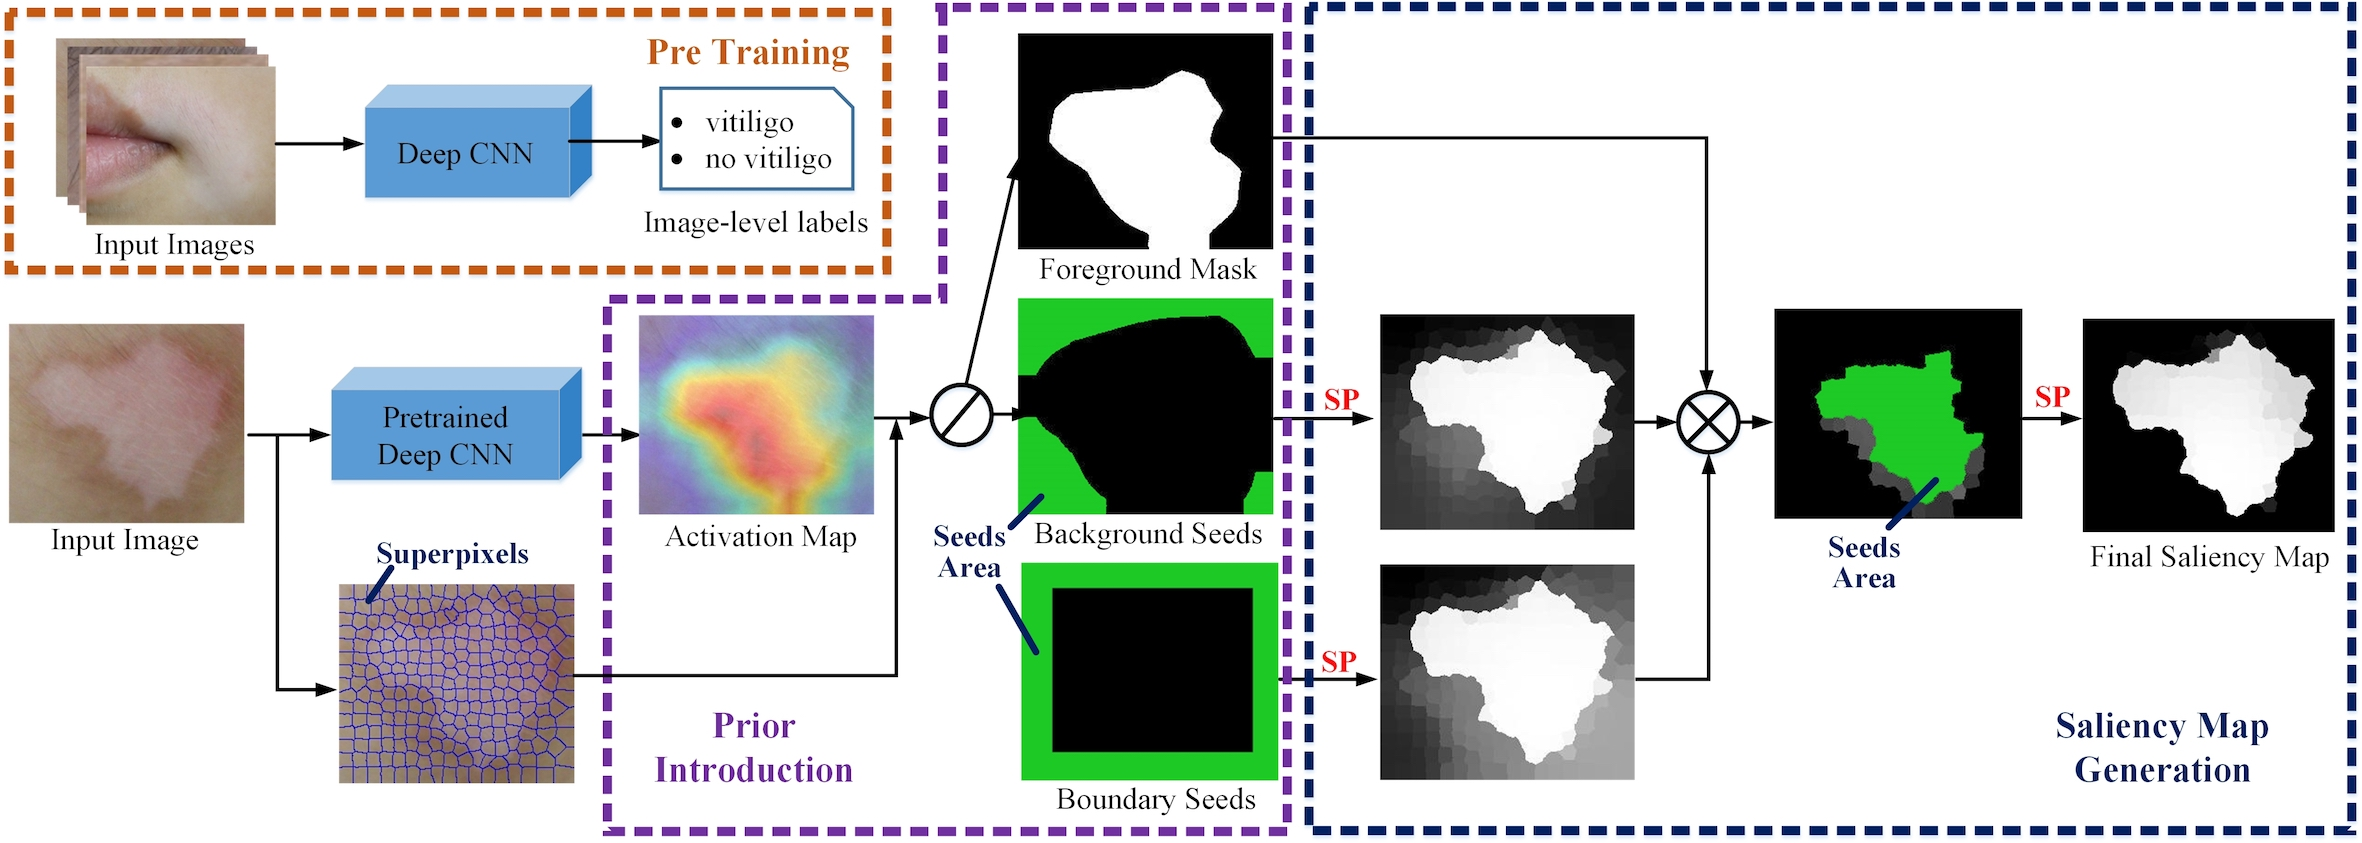
\includegraphics[width=\linewidth]{figures/CNNandSuperPixelModelGraph3.jpg}
\end{figure}
\begin{itemize}
\item 边界先验(Boundary Prior): 假设边界为背景区域
\item 三次显著性传播过程({\color{red}SP})
\end{itemize}
\end{frame}



























